\documentclass{article}

\usepackage{graphicx}
\usepackage{tikz}
\usepackage{tikzsymbols}
\usetikzlibrary{calc,patterns,shapes.geometric}
\pagestyle{empty}
\usepackage[margin=0pt]{geometry}
\geometry{papersize={14in,12in}}

\def\centerarc[#1](#2)(#3:#4:#5){\draw[#1] ($(#2)+({#5*cos(#3)},{#5*sin(#3)})$) arc (#3:#4:#5);}

\begin{document}
	\begin{figure}
		\centering
		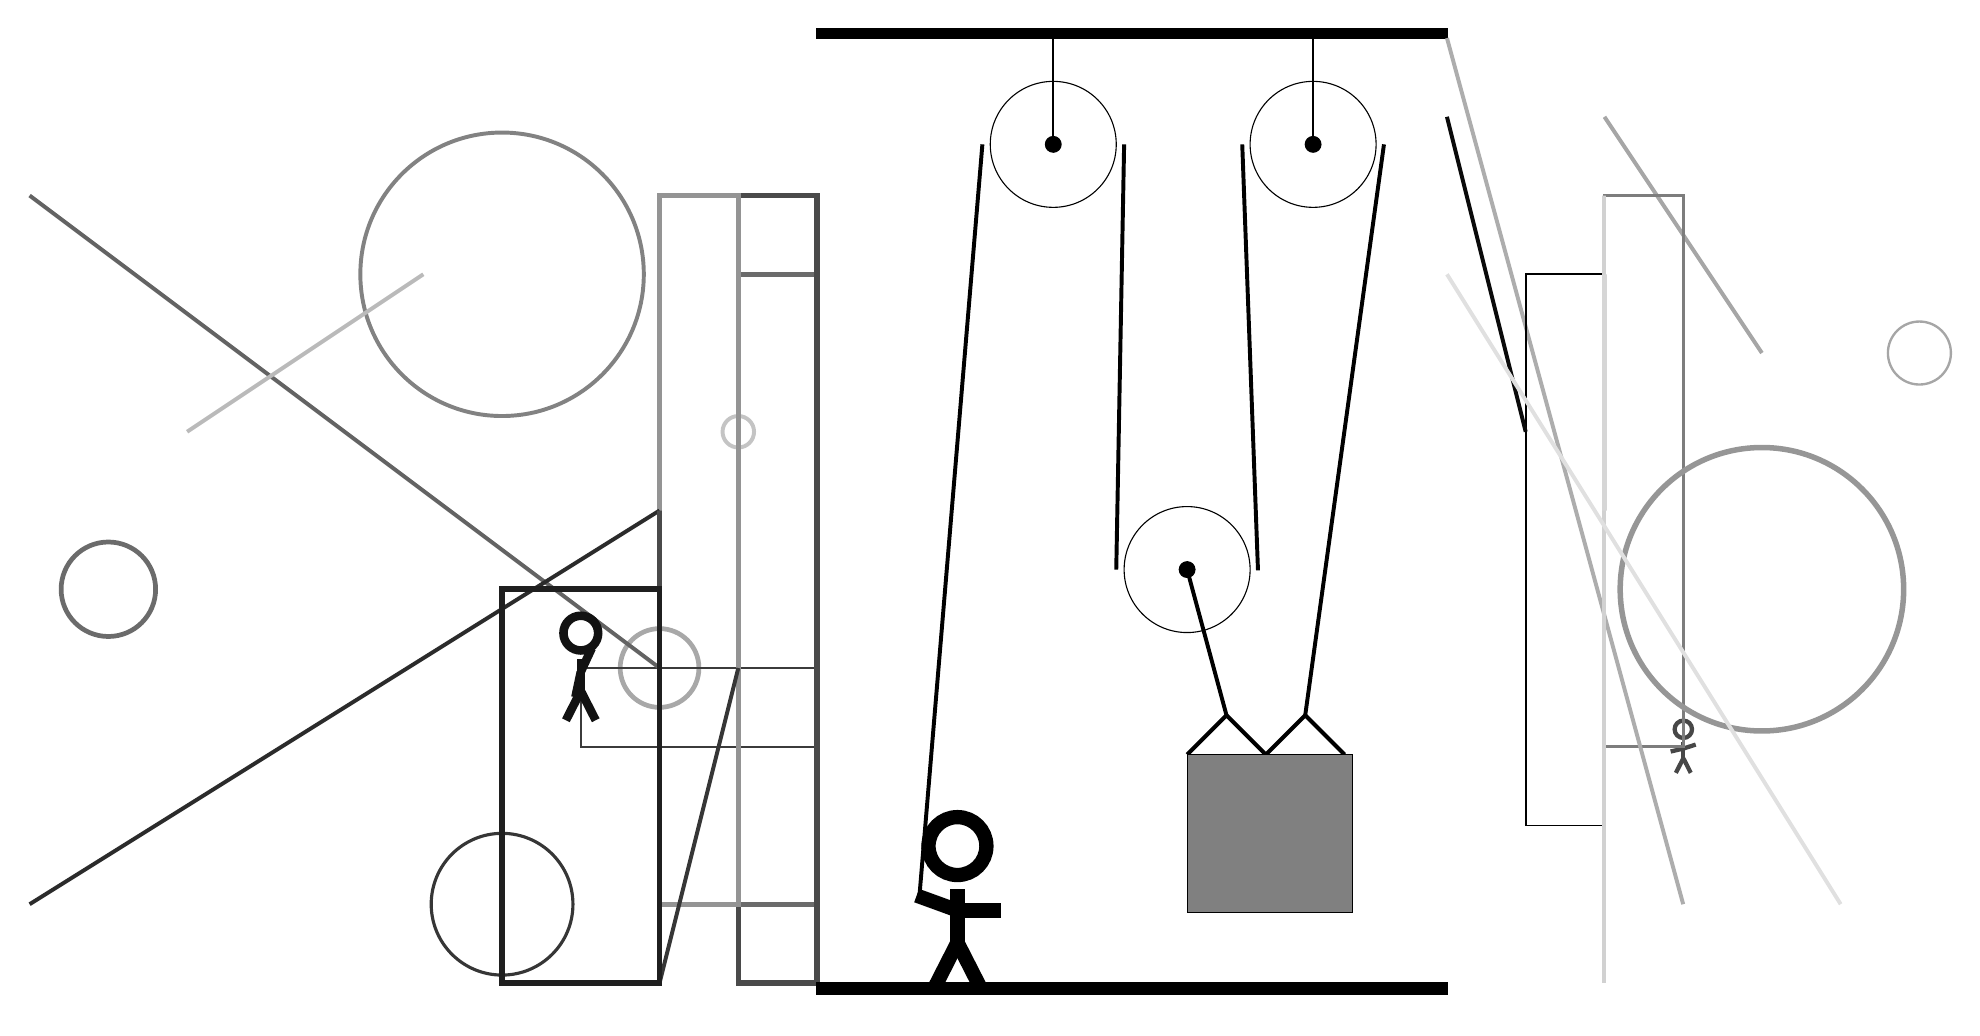
\begin{tikzpicture}
			%%%%% START %%%%%
			
			\draw[fill=black] (-2, 9) rectangle (6, 9.125);
			
			\draw (1, 7.65) circle (0.8);
			\draw[fill=black] (1, 7.65) circle (0.1);
			\draw[thick] (1, 7.65) -- (1, 9);
			
			\draw (4.3, 7.65) circle (0.8);
			\draw[fill=black] (4.3, 7.65) circle (0.1);
			\draw[thick] (4.3, 7.65) -- (4.3, 9);
			
			\draw (2.7, 2.25) circle (0.8);
			\draw[fill=black] (2.7, 2.25) circle (0.1);
			
			\draw[line width=0.5mm]  (2.7, -0.1) -- (3.2, 0.4) -- (3.7, -0.1) -- (4.2, 0.4) -- (4.7, -0.1);
			\draw[fill=black!50] (2.7, -0.1) rectangle (4.8, -2.1);
			
			\draw[line width=0.5mm](-0.7, -1.9) -- (0.1, 7.65);
			\centerarc[line width=0.5mm](1, 7.65)(0:180:0.9);
			\draw[line width=0.5mm](1.9, 7.65) -- (1.8, 2.25);
			\centerarc[line width=0.5mm](2.7, 2.25)(180:370:0.9);
			\draw[line width=0.5mm] (3.6, 2.24) -- (3.4, 7.65);
			\centerarc[line width=0.5mm](4.3, 7.65)(0:180:0.9);
			\draw[line width=0.5mm](4.2, 0.4) -- (5.2, 7.65);
			\draw[line width=0.5mm] (3.2, 0.4) -- (2.7, 2.25);
			
			\draw [line width=0.5mm, color=black!23](-3, 4) circle (0.2);
			
			\draw [line width=0.5mm, color=black!49](-6, 6) circle (1.8);
			\draw[line width=0.5mm, color=black!35](8, 8) -- (10, 5);
			\node[line width=0.7mm, color=black!72] at (9, 0) {\Strichmaxerl[3][13][18]};
			\draw [line width=0.4mm, color=black!79](-6, -2) circle (0.9);
			\draw [line width=0.6mm, color=black!34](-4, 1) circle (0.5);
			\draw[line width=0.2mm, color=black!77] (-2, 0) rectangle (-5, 1);
			\draw [line width=0.3mm, color=black!35](12, 5) circle (0.4);
			\draw[line width=0.5mm, color=black!61](-4, 1) -- (-12, 7);
			\draw [line width=0.6mm, color=black!58](-11, 2) circle (0.6);
			\draw[line width=0.4mm, color=black!51] (8, 0) rectangle (9, 7);
			\draw[line width=0.5mm, color=black!32](6, 9) -- (9, -2);
			\node[line width=0.3mm, color=black!93] at (-5, 1) {\Strichmaxerl[6][78][65]};
			
			\draw[line width=0.6mm, color=black!58] (-3, -2) rectangle (-2, 6);
			\draw[line width=0.2mm, color=black!100] (7, 6) rectangle (8, -1);
			\draw[line width=0.7mm, color=black!71] (-2, -3) rectangle (-3, 7);
			
			\draw[line width=0.6mm, color=black!42] (-3, 7) rectangle (-4, -2);
			\draw [line width=0.7mm, color=black!41](10, 2) circle (1.8);
			\draw[line width=0.5mm, color=black!18] (8, -3) rectangle (8, 7);
			\draw[line width=0.5mm, color=black!83](-4, 3) -- (-12, -2);
			\draw[line width=0.7mm, color=black!71] (-4, 1) rectangle (-4, 3);
			
			\draw[line width=0.5mm, color=black!27](-7, 6) -- (-10, 4);
			\draw[line width=0.7mm, color=black!16] (8, 3) rectangle (8, 6);
			\draw[line width=0.5mm, color=black!96](7, 4) -- (6, 8);
			\draw[line width=0.5mm, color=black!79](-4, -3) -- (-3, 1);
			
			\draw[line width=0.7mm, color=black!88] (-4, 2) rectangle (-6, -3);
			\draw[line width=0.5mm, color=black!12](11, -2) -- (6, 6);
			
			\node at (-0.2, -2) {\Strichmaxerl[10][-20][0]};
			
			\draw[fill=black] (-2, -3) rectangle (6, -3.15);
			
			%%%%% END %%%%%
		\end{tikzpicture}
	\end{figure}	
\end{document}